% !TeX program = xelatex
\documentclass[a4paper,10pt]{article}

% ============================================================================
% កញ្ចប់បណ្ណាល័យ (Packages) – តាមលំនាំ NGS Preah Krasang (ls_plan.tex)
% ============================================================================
\usepackage[a4paper, left=0.95cm, right=0.95cm, top=0.85cm, bottom=0.92cm, footskip=0.52cm]{geometry}
\usepackage{amsmath, amssymb}
\usepackage{unicode-math}
\usepackage{fontspec}
\usepackage{array, longtable, multirow, colortbl}
\usepackage[table]{xcolor}
\usepackage{enumitem}
\usepackage{pifont}
\usepackage{fancyhdr}
\usepackage{tikz}
\usetikzlibrary{calc, arrows.meta, angles, quotes, decorations.markings, positioning, babel}

% LaTeX 2025 + longtable v4.24 compatibility guard
\makeatletter
\let\@expl@@@mark@update@singlecol@structures@@\relax
\makeatother

% ============================================================================
% ការកំណត់ពុម្ពអក្សរ (Fonts Configuration - Cross-Platform Windows + Cloud fonts/)
% ============================================================================
\providecommand{\NGSFindFonts}{%
  \IfFileExists{C:/Windows/Fonts/cambria.ttc}{%
    \def\NGSSysPath{C:/Windows/Fonts/}%
    \def\NGSUserPath{C:/Users/KIT/AppData/Local/Microsoft/Windows/Fonts/}%
  }{%
    \IfFileExists{./fonts/KhmerOSsiemreap.ttf}{\def\NGSSysPath{./fonts/}\def\NGSUserPath{./fonts/}}{%
    \IfFileExists{../fonts/KhmerOSsiemreap.ttf}{\def\NGSSysPath{../fonts/}\def\NGSUserPath{../fonts/}}{%
    \IfFileExists{../../fonts/KhmerOSsiemreap.ttf}{\def\NGSSysPath{../../fonts/}\def\NGSUserPath{../../fonts/}}{%
    \IfFileExists{../../../fonts/KhmerOSsiemreap.ttf}{\def\NGSSysPath{../../../fonts/}\def\NGSUserPath{../../../fonts/}}{%
    \IfFileExists{../../../../fonts/KhmerOSsiemreap.ttf}{\def\NGSSysPath{../../../../fonts/}\def\NGSUserPath{../../../../fonts/}}{%
    \IfFileExists{../../../../../fonts/KhmerOSsiemreap.ttf}{\def\NGSSysPath{../../../../../fonts/}\def\NGSUserPath{../../../../../fonts/}}{%
    \IfFileExists{../../../../../../fonts/KhmerOSsiemreap.ttf}{\def\NGSSysPath{../../../../../../fonts/}\def\NGSUserPath{../../../../../../fonts/}}{%
      \def\NGSSysPath{../../../../../../../fonts/}\def\NGSUserPath{../../../../../../../fonts/}%
    }}}}}}}%
  }%
}
\NGSFindFonts

\setmathfont[
  Path={\NGSSysPath},
  FontIndex=1,
  Scale=1.02
]{cambria.ttc}

\defaultfontfeatures{Ligatures=TeX}

\setmainfont[
  Path={\NGSUserPath},
  Extension=.ttf,
  Script=Khmer,
  BoldFont={KhmerOSsiemreap},
  BoldFeatures={FakeBold=1.8},
  ItalicFont={KhmerOSsiemreap},
  ItalicFeatures={FakeSlant=0.25},
  BoldItalicFont={KhmerOSsiemreap},
  BoldItalicFeatures={FakeBold=1.8, FakeSlant=0.25}
]{KhmerOSsiemreap}

\newfontfamily\muol[
  Path={\NGSUserPath},
  Extension=.ttf,
  Script=Khmer
]{KhmerOSmuollight}

\newfontfamily\TimesEn[
  Path={\NGSSysPath},
  Extension=.ttf,
  Scale=1.00,
  BoldFont={timesbd},
  ItalicFont={timesi},
  BoldItalicFont={timesbi}
]{times}

\newfontfamily\NagaBold[
  Path={\NGSUserPath},
  Extension=.ttf
]{AKbalthom Naga Bold}

\newfontfamily\CalibriFont[
  Path={\NGSSysPath},
  Extension=.ttf
]{calibri}

\newfontfamily\Tacteing[
  Path={\NGSUserPath}
]{TACTENG.TTF}

\newfontfamily\CourierBullet[
  Path={\NGSSysPath},
  Extension=.ttf
]{cour}
\newcommand{\wcirc}{{\CourierBullet\fontsize{9.5pt}{11pt}\selectfont o}}

% ក្បួនកាត់ពាក្យខ្មែរ (Khmer word wrapping)
\XeTeXlinebreaklocale "km"
\XeTeXlinebreakskip = 0pt plus 1pt minus 0.1pt

% ============================================================================
% ការកំណត់ពណ៌ និងទម្រង់ទំព័រ (Colors & Page Style)
% ============================================================================
\definecolor{stepgray}{HTML}{D9D9D9}
\definecolor{headgray}{HTML}{F2F2F2}
\definecolor{boxgray}{HTML}{D9D9D9}
\definecolor{darkred}{HTML}{C00000}
\definecolor{red5e}{HTML}{FF0000}

\pagestyle{fancy}
\fancyhf{}
\renewcommand{\headrulewidth}{0pt}
\fancyfoot[R]{\CalibriFont\fontsize{11pt}{13pt}\selectfont\thepage}

\setlength{\parindent}{0pt}
\setlength{\parskip}{0pt}
\setlength{\tabcolsep}{3.8pt}

\newcolumntype{L}[1]{>{\raggedright\arraybackslash}p{#1}}
\newcolumntype{C}[1]{>{\centering\arraybackslash}p{#1}}

% ============================================================================
% ម៉ាក្រូជំនួយ (Helper Macros)
% ============================================================================
\newcommand{\en}[1]{{\TimesEn #1}}
\newcommand{\enbf}[1]{{\TimesEn\textbf{#1}}}
\newcommand{\unit}[1]{\,\text{\en{#1}}}
\newcommand{\fiveE}[1]{{\NagaBold\fontsize{9.5pt}{13pt}\selectfont\textcolor{red5e}{#1}}}
\newcommand{\timenote}[1]{\textcolor{darkred}{\textit{#1}}}
\newcommand{\redsub}[1]{\textcolor{darkred}{#1}}
\newcommand{\graybox}[1]{\colorbox{boxgray}{\strut\hspace{2pt}#1\hspace{2pt}}}
\newcommand{\ditem}{\tikz[baseline=-0.5ex]\fill (0,0.42ex) -- (0.42ex,0) -- (0,-0.42ex) -- (-0.42ex,0) -- cycle;\hspace{0.3em}}
\newcommand{\cnum}[1]{{\TimesEn\fontsize{10.5pt}{12pt}\selectfont\ding{\numexpr181+#1\relax}}\hspace{0.2em}}
\newcommand{\cfig}[1]{\par\vspace{4pt}{\centering #1\par}\vspace{4pt}}
\newcommand{\stepheader}[1]{\multicolumn{3}{|c|}{\cellcolor{stepgray}\muol #1} \\* \noalign{\hrule height 0.4pt}}
\newcommand{\fstrut}{\rule[-2.1ex]{0pt}{5.4ex}}

% ក្បាច់ក្រោមបាវចនា (Tacteing Font - Keyboard '3')
\newcommand{\khmflourish}{{\Tacteing\fontsize{36pt}{14pt}\selectfont\raisebox{-5pt}{3}}}

% រចនាប័ទ្មគូសសម្គាល់ B&W Print-Safe
\tikzset{
  tk1/.style={postaction={decorate},decoration={markings,mark=at position 0.50 with {\draw[black, line width=0.85pt](0,-0.095)--(0,0.095);}}},
  tk2/.style={postaction={decorate},decoration={markings,
    mark=at position 0.45 with {\draw[black, line width=0.85pt](0,-0.095)--(0,0.095);},
    mark=at position 0.55 with {\draw[black, line width=0.85pt](0,-0.095)--(0,0.095);}}},
  traceArr/.style={black, densely dashed, line width=0.9pt, -{Stealth[length=4pt]}}
}

% ============================================================================
% ម៉ាក្រូគូសរូប TikZ ស-ខ្មៅ សមាមាត្រធំច្បាស់ (4.8cm–7.0cm, font=\footnotesize, text=black)
% ============================================================================

% រូបទី១៖ បន្ទាត់ចំនួនផ្ទៀងផ្ទាត់កំណែកិច្ចការផ្ទះមេរៀន ២.២ (ទទឹង ~6.8 cm ក្នុង Col 2)
\newcommand{\figHWRevRAT}{%
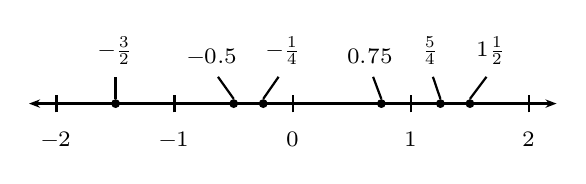
\begin{tikzpicture}[x=1cm, y=1cm, every node/.style={font=\footnotesize, text=black}]
  \draw[{Stealth[length=4pt]}-{Stealth[length=4pt]}, black, line width=0.95pt] (-3.35,0) -- (3.35,0);
  \foreach \x/\lbl in {-3.0/-2, -1.5/-1, 0/0, 1.5/1, 3.0/2} {
    \draw[black, line width=0.85pt] (\x,-0.11) -- (\x,0.11);
    \node[below=3.5pt] at (\x,-0.11) {$\lbl$};
  }
  % ចំណុចទាំង ៦៖ -3/2 (-2.25), -0.5 (-0.75), -1/4 (-0.375), 0.75 (1.125), 5/4 (1.875), 1 1/2 (2.25)
  \fill[black] (-2.25,0) circle (1.6pt);
  \draw[black, line width=0.8pt] (-2.25,0.06) -- (-2.25,0.34);
  \node[above=1pt] at (-2.25,0.34) {$-\frac{3}{2}$};

  \fill[black] (-0.75,0) circle (1.6pt);
  \draw[black, line width=0.8pt] (-0.75,0.06) -- (-0.95,0.34);
  \node[above=1pt] at (-1.02,0.34) {$-0.5$};

  \fill[black] (-0.375,0) circle (1.6pt);
  \draw[black, line width=0.8pt] (-0.375,0.06) -- (-0.18,0.34);
  \node[above=1pt] at (-0.12,0.34) {$-\frac{1}{4}$};

  \fill[black] (1.125,0) circle (1.6pt);
  \draw[black, line width=0.8pt] (1.125,0.06) -- (1.02,0.34);
  \node[above=1pt] at (0.98,0.34) {$0.75$};

  \fill[black] (1.875,0) circle (1.6pt);
  \draw[black, line width=0.8pt] (1.875,0.06) -- (1.78,0.34);
  \node[above=1pt] at (1.75,0.34) {$\frac{5}{4}$};

  \fill[black] (2.25,0) circle (1.6pt);
  \draw[black, line width=0.8pt] (2.25,0.06) -- (2.46,0.34);
  \node[above=1pt] at (2.52,0.34) {$1\frac{1}{2}$};
\end{tikzpicture}}

% រូបទី២៖ បង្គោលវាស់កម្ពស់ទឹកក្រោមស្ពានកំពង់ស្វាយ (ទិសឈរ + បន្ទះជញ្ជីងផ្អៀង ~140° មិនស្ដង់ដារ, ~6.8 cm)
\newcommand{\figGaugeHookEOne}{%
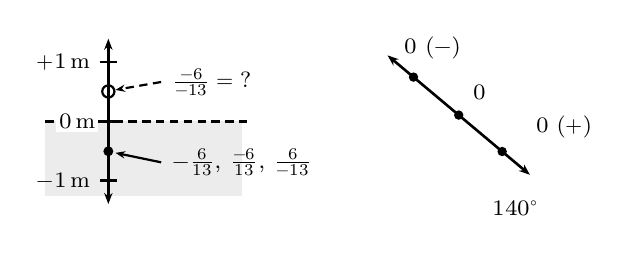
\begin{tikzpicture}[x=1cm, y=1cm, every node/.style={font=\footnotesize, text=black}]
  % ឆ្វេង៖ បង្គោលវាស់ទឹកទិសឈរ
  \begin{scope}[shift={(-1.85,0)}]
    \fill[gray!15] (-1.35,-0.95) rectangle (1.15,0);
    \draw[black, densely dashed, line width=0.85pt] (-1.35,0) -- (1.25,0);
    \draw[{Stealth[length=4pt]}-{Stealth[length=4pt]}, black, line width=1.05pt] (-0.55,-1.05) -- (-0.55,1.05);
    \draw[black, line width=0.85pt] (-0.66,0.75) -- (-0.44,0.75) node[left=6pt] {$+1\unit{m}$};
    \draw[black, line width=0.95pt] (-0.68,0) -- (-0.42,0) node[left=7pt, fill=white, inner sep=1pt] {$0\unit{m}$};
    \draw[black, line width=0.85pt] (-0.66,-0.75) -- (-0.44,-0.75) node[left=6pt] {$-1\unit{m}$};
    % កម្រិតទឹកក្រោមសូន្យ (-6/13) និងលើសូន្យ (+6/13)
    \fill[black] (-0.55,-0.38) circle (1.8pt);
    \draw[black, line width=0.8pt, -{Stealth[length=3.5pt]}] (0.12,-0.52) -- (-0.46,-0.40);
    \node[right=1pt] at (0.10,-0.52) {$-\frac{6}{13},\,\frac{-6}{13},\,\frac{6}{-13}$};
    \draw[black, line width=0.8pt] (-0.55,0.38) circle (2.2pt);
    \draw[black, densely dashed, line width=0.8pt, -{Stealth[length=3.5pt]}] (0.12,0.50) -- (-0.46,0.40);
    \node[right=1pt] at (0.10,0.50) {$\frac{-6}{-13}=\text{?}$};
  \end{scope}
  % ស្ដាំ៖ បន្ទាត់ចំនួនផ្អៀង 140° (បំបែកទម្លាប់មើលតែបន្ទាត់ដេក)
  \begin{scope}[shift={(2.05,0.08)}]
    \draw[{Stealth[length=4pt]}-{Stealth[length=4pt]}, black, line width=0.95pt] (140:1.18) -- (-40:1.18);
    \fill[black] (0,0) circle (1.7pt);
    \node[above right=2.5pt] at (0,0) {$0$};
    \fill[black] (140:0.75) circle (1.7pt);
    \node[above=3pt] at (140:0.75) {ក្រោម $0$ ($-$)};
    \fill[black] (-40:0.72) circle (1.7pt);
    \node[above right=2pt] at (-40:0.72) {លើ $0$ ($+$)};
    \node at (0,-1.18) {អ័ក្សរង្វាស់ផ្អៀង $140^\circ$};
  \end{scope}
\end{tikzpicture}}

% រូបទី៣៖ បន្ទះប្រភាគសមមូល 5/7 = -25/-35 និងបន្ទាត់ចំនួនឆ្លុះសញ្ញាដក (ទទឹង ~6.8 cm)
\newcommand{\figExploreStripsETwo}{%
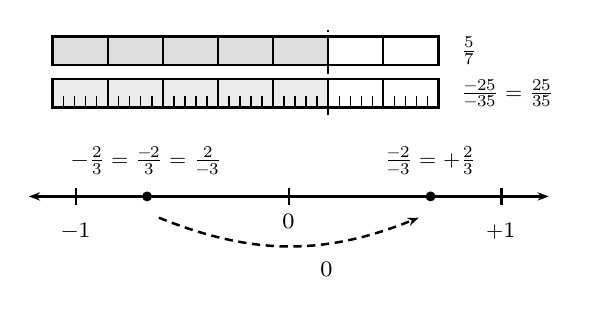
\begin{tikzpicture}[x=1cm, y=1cm, every node/.style={font=\footnotesize, text=black}]
  % បន្ទះលើ៖ 5/7 ធៀប 25/35 = (-25)/(-35)
  \fill[gray!26] (0,1.22) rectangle (3.50,1.58);
  \draw[black, line width=0.9pt] (0,1.22) rectangle (4.90,1.58);
  \foreach \k in {1,...,6} {
    \draw[black, line width=0.8pt] ({0.70*\k},1.22) -- ({0.70*\k},1.58);
  }
  \node[right=4pt] at (4.92,1.40) {$\frac{5}{7}$};

  \fill[gray!16] (0,0.68) rectangle (3.50,1.04);
  \draw[black, line width=0.9pt] (0,0.68) rectangle (4.90,1.04);
  \foreach \k in {1,...,6} {
    \draw[black, line width=0.85pt] ({0.70*\k},0.68) -- ({0.70*\k},1.04);
  }
  \foreach \m in {1,...,34} {
    \draw[black, line width=0.5pt] ({0.14*\m},0.68) -- ({0.14*\m},0.82);
  }
  \draw[black, densely dashed, line width=0.85pt] (3.50,0.58) -- (3.50,1.66);
  \node[right=4pt] at (4.92,0.86) {$\frac{-25}{-35}=\frac{25}{35}$};

  % បន្ទាត់ចំនួនខាងក្រោម៖ ឆ្លុះរវាង -2/3 និង (-2)/(-3) = +2/3
  \draw[{Stealth[length=4pt]}-{Stealth[length=4pt]}, black, line width=0.95pt] (-0.30,-0.45) -- (6.30,-0.45);
  \foreach \x/\lbl in {0.30/-1, 5.70/+1} {
    \draw[black, line width=0.85pt] (\x,-0.56) -- (\x,-0.34);
    \node[below=3pt] at (\x,-0.56) {$\lbl$};
  }
  \draw[black, line width=0.9pt] (3.00,-0.56) -- (3.00,-0.34);
  \node[below=2pt, fill=white, inner sep=1pt] at (3.00,-0.56) {$0$};
  \fill[black] (1.20,-0.45) circle (1.8pt);
  \node[above=3pt] at (1.20,-0.40) {$-\frac{2}{3}=\frac{-2}{3}=\frac{2}{-3}$};
  \fill[black] (4.80,-0.45) circle (1.8pt);
  \node[above=3pt] at (4.80,-0.40) {$\frac{-2}{-3}=+\frac{2}{3}$};
  \draw[traceArr] (1.35,-0.72) to[bend right=22] node[below=2pt] {ឆ្លុះធៀបគល់ $0$} (4.65,-0.72);
\end{tikzpicture}}

% រូបទី៤៖ អន្ទាក់ POE 2B — ហេតុអ្វីវិសមភាពផលគុណខ្វែងត្រូវការ b>0 និង d>0? (~7.55 cm)
\newcommand{\figInequalityTrapETwo}{%
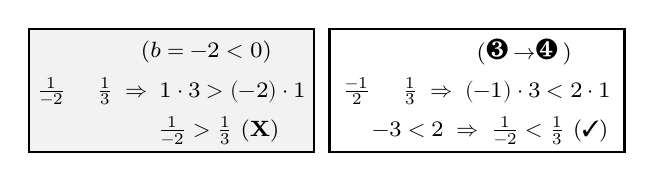
\begin{tikzpicture}[x=1cm, y=1cm, every node/.style={font=\footnotesize, text=black}]
  % ឆ្វេង៖ អន្ទាក់ខុសពេល b=-2 < 0
  \draw[black, line width=0.85pt, fill=gray!10] (0,0) rectangle (3.62,1.56);
  \node at (1.81,1.27) {\textbf{អន្ទាក់ខុស} ($b=-2<0$)};
  \node at (1.81,0.77) {$\frac{1}{-2}\;\text{និង}\;\frac{1}{3}\;\Rightarrow\;1\cdot 3 > (-2)\cdot 1$};
  \node at (1.81,0.27) {សន្និដ្ឋានខុស៖ $\frac{1}{-2}>\frac{1}{3}$ (\enbf{X})};

  % ស្ដាំ៖ វិធីត្រឹមត្រូវ ប្ដូរភាគបែងវិជ្ជមានមុន (③ -> ④)
  \draw[black, line width=0.95pt, fill=white] (3.82,0) rectangle (7.56,1.56);
  \node at (5.69,1.27) {\textbf{វិធីត្រឹមត្រូវ} (\cnum{3}$\to$\cnum{4})};
  \node at (5.69,0.77) {$\frac{-1}{2}\;\text{និង}\;\frac{1}{3}\;\Rightarrow\;(-1)\cdot 3 < 2\cdot 1$};
  \node at (5.69,0.27) {បាន $-3<2\;\Rightarrow\;\frac{1}{-2}<\frac{1}{3}$ (\ding{51})};
\end{tikzpicture}}

% រូបទី៥៖ រចនាសម្ព័ន្ធគំនិត Hub-and-Spoke នៃលក្ខណៈចំនួនសនិទាន និងធនាគារហេតុផល ①–⑤ (~6.9 cm)
\newcommand{\figHubSpokeEThree}{%
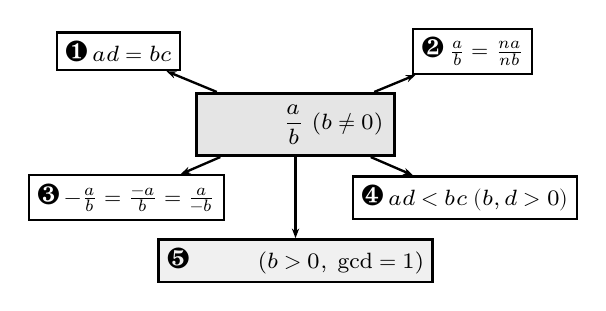
\begin{tikzpicture}[x=1cm, y=1cm, every node/.style={font=\footnotesize, text=black}]
  \node[draw=black, line width=1.0pt, fill=gray!20, inner sep=4pt, align=center] (hub) at (0,0.15)
    {\textbf{ស្នូលសនិទាន} $\dfrac{a}{b}$ ($b\neq 0$)};
  \node[draw=black, line width=0.8pt, fill=white, inner sep=3pt] (s1) at (-2.25,1.08) {\cnum{1}$ad=bc$};
  \node[draw=black, line width=0.8pt, fill=white, inner sep=3pt] (s2) at (2.25,1.08) {\cnum{2}$\frac{a}{b}=\frac{na}{nb}$};
  \node[draw=black, line width=0.8pt, fill=white, inner sep=3pt] (s3) at (-2.15,-0.78) {\cnum{3}$-\frac{a}{b}=\frac{-a}{b}=\frac{a}{-b}$};
  \node[draw=black, line width=0.8pt, fill=white, inner sep=3pt] (s4) at (2.15,-0.78) {\cnum{4}$ad<bc\;(b,d>0)$};
  \node[draw=black, line width=0.85pt, fill=gray!12, inner sep=3pt] (s5) at (0,-1.58) {\cnum{5}បង្រួមរួច ($b>0,\;\gcd=1$)};
  \draw[black, line width=0.85pt, -{Stealth[length=3.5pt]}] (hub) -- (s1);
  \draw[black, line width=0.85pt, -{Stealth[length=3.5pt]}] (hub) -- (s2);
  \draw[black, line width=0.85pt, -{Stealth[length=3.5pt]}] (hub) -- (s3);
  \draw[black, line width=0.85pt, -{Stealth[length=3.5pt]}] (hub) -- (s4);
  \draw[black, line width=0.85pt, -{Stealth[length=3.5pt]}] (hub) -- (s5);
\end{tikzpicture}}

% រូបទី៦៖ គំនូសសញ្ញា ស-ខ្មៅ + [tracing] អូសខ្វែងលើលំហាត់គំរូ គ (-15/36 និង 20/-48) (~6.8 cm)
\newcommand{\figDetectiveCardEFour}{%
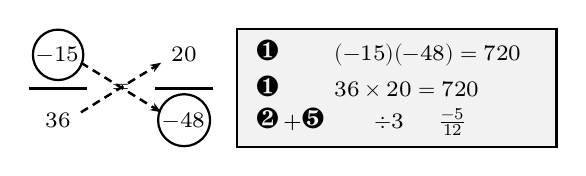
\begin{tikzpicture}[x=1cm, y=1cm, every node/.style={font=\footnotesize, text=black}]
  % ផ្នែកឆ្វេង៖ ផលគុណខ្វែង [tracing]
  \node (n1) at (0.45,0.95) {$-15$};
  \draw[black, line width=0.8pt] (0.45,0.95) circle (0.32cm);
  \draw[black, line width=0.9pt] (0.08,0.52) -- (0.82,0.52);
  \node (d1) at (0.45,0.12) {$36$};

  \node at (1.25,0.52) {$=$};

  \node (n2) at (2.05,0.95) {$20$};
  \draw[black, line width=0.9pt] (1.68,0.52) -- (2.42,0.52);
  \node (d2) at (2.05,0.12) {$-48$};
  \draw[black, line width=0.8pt] (2.05,0.12) circle (0.33cm);

  \draw[traceArr] (0.74,0.85) -- (1.76,0.22);
  \draw[traceArr] (0.74,0.22) -- (1.76,0.85);

  % ផ្នែកស្ដាំ៖ សង្ខេបជំហានស៊ើបអង្កេត ៣ ជំហាន
  \draw[black, line width=0.85pt, fill=gray!10] (2.72,-0.22) rectangle (6.78,1.28);
  \node[anchor=west] at (2.84,0.98) {\cnum{1}ខ្វែង១៖ $(-15)(-48)=720$};
  \node[anchor=west] at (2.84,0.55) {\cnum{1}ខ្វែង២៖ $36\times 20=720$};
  \node[anchor=west] at (2.84,0.10) {\cnum{2}+\cnum{5}សម្រួល $\div 3$ បាន $\frac{-5}{12}$};
\end{tikzpicture}}

% រូបទី៧៖ ក្បួនរាប់សញ្ញាដកគូ-សេសលើលំហាត់ ១ (ទំព័រ ១១ — អ្នកប្រមាញ់តម្លៃ -5, ~7.25 cm)
\newcommand{\figOddSignHunterEFive}{%
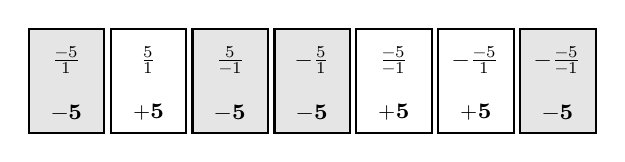
\begin{tikzpicture}[x=1cm, y=1cm, every node/.style={font=\footnotesize, text=black}]
  \foreach \i/\expr/\res/\sh in {
    0/{\frac{-5}{1}}/{-5}/gray!20,
    1/{\frac{5}{1}}/{+5}/white,
    2/{\frac{5}{-1}}/{-5}/gray!20,
    3/{-\frac{5}{1}}/{-5}/gray!20,
    4/{\frac{-5}{-1}}/{+5}/white,
    5/{-\frac{-5}{1}}/{+5}/white,
    6/{-\frac{-5}{-1}}/{-5}/gray!20} {
    \draw[black, line width=0.8pt, fill=\sh] ({1.04*\i},0) rectangle ({1.04*\i+0.96},1.32);
    \node at ({1.04*\i+0.48},0.92) {$\expr$};
    \node at ({1.04*\i+0.48},0.26) {$\mathbf{\res}$};
  }
\end{tikzpicture}}

% រូបទី៨៖ គំនូសសុវត្ថិភាព ③ -> ④ សម្រាប់កិច្ចការផ្ទះ ខ.២ (5/(-8) ធៀប -3/5, ~5.8 cm)
\newcommand{\figHomeworkSafetyGate}{%
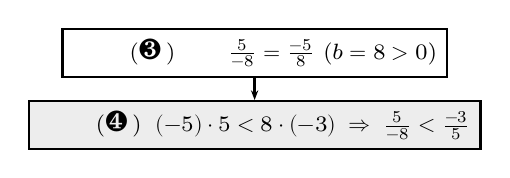
\begin{tikzpicture}[x=1cm, y=1cm, every node/.style={font=\footnotesize, text=black}]
  \node[draw=black, line width=0.8pt, fill=white, inner sep=3.5pt] (a) at (0,0.92)
    {ជំហានទី១ (\cnum{3})៖ ប្ដូរ $\frac{5}{-8}=\frac{-5}{8}$ ($b=8>0$)};
  \node[draw=black, line width=0.85pt, fill=gray!14, inner sep=3.5pt] (b) at (0,0)
    {ជំហានទី២ (\cnum{4})៖ $(-5)\cdot 5 < 8\cdot(-3)\;\Rightarrow\;\frac{5}{-8}<\frac{-3}{5}$};
  \draw[black, line width=0.85pt, -{Stealth[length=3.5pt]}] (a) -- (b);
\end{tikzpicture}}

% ============================================================================
% ចាប់ផ្ដើមឯកសារ (Document Body — ចំនួនទំព័រតាមខ្លឹមសារជាក់ស្ដែង, ពេញទំព័រ >=90%)
% ============================================================================
\begin{document}
\fontsize{10pt}{15.2pt}\selectfont

% -------------------- ក្បាលកិច្ចតែងការ (Header) --------------------
\begin{center}
  {\muol\fontsize{11pt}{16pt}\selectfont ព្រះរាជាណាចក្រកម្ពុជា}\\[2pt]
  {\muol\fontsize{10pt}{15pt}\selectfont ជាតិ សាសនា ព្រះមហាក្សត្រ}\\[1pt]
  \khmflourish
\end{center}

\vspace{-15pt}
{\muol\fontsize{9.5pt}{13.2pt}\selectfont
មន្ទីរអប់រំ យុវជន និងកីឡា ខេត្តកំពង់ធំ\\
ការិយាល័យអប់រំ យុវជន និងកីឡា ស្រុកកំពង់ស្វាយ\\
អនុវិទ្យាល័យព្រះក្រសាំង}

\vspace{2pt}
\begin{center}
  {\muol\fontsize{10pt}{15pt}\selectfont កិច្ចតែងការបង្រៀន}
\end{center}
\vspace{1pt}

% -------------------- ព័ត៌មានទូទៅ (Metadata) --------------------
{\renewcommand{\arraystretch}{1.06}
\hspace*{4.6cm}%
\begin{tabular}{@{}l l l@{}}
  - \hspace{0.35cm} មុខវិជ្ជា & : & គណិតវិទ្យា ថ្នាក់ទី៨ (ពីជគណិត) \\
  - \hspace{0.35cm} ចំណងជើងមេរៀន & : & មេរៀនទី១៖ ចំនួនសនិទាន \\
  - \hspace{0.35cm} ចំណងជើងរង & : & ២.៣. លក្ខណៈនៃចំនួនសនិទាន (ទំព័រ ៥ និងលំហាត់ ១ ទំព័រ ១១) \\
  - \hspace{0.35cm} រយៈពេល & : & ១ ម៉ោងសិក្សា (៥០នាទី) \\
  - \hspace{0.35cm} បង្រៀនដោយ & : & ហុក ប៊ុនថែន \\
  - \hspace{0.35cm} កាលបរិច្ឆេទ & : & ថ្ងៃចន្ទ ទី១៦ ខែវិច្ឆិកា ឆ្នាំ២០២៦ \\
\end{tabular}

\vspace{2pt}

% -------------------- I. វត្ថុបំណង --------------------
\textbf{I.} {\muol វត្ថុបំណង}\\[2pt]
\hspace*{0.55cm}%
\begin{tabular}{@{}l l L{14.2cm}@{}}
  \wcirc \hspace{0.25cm} វិជ្ជាសម្បទា & : & សិស្សប្រាប់បានពីលក្ខណៈទាំង ៤ នៃចំនួនសនិទាន ($\frac{a}{b}=\frac{c}{d}\Leftrightarrow ad=bc$, $\frac{a}{b}=\frac{na}{nb}$, $-\frac{a}{b}=\frac{-a}{b}=\frac{a}{-b}$, និងវិសមភាព $ad<bc$ ចំពោះ $b>0, d>0$) ព្រមទាំងនិយមន័យទម្រង់បង្រួមរួចស្ដង់ដារបានត្រឹមត្រូវតាមរយៈការពិសោធបន្ទះប្រភាគ និងតារាងសំយោគ។ \\
  \wcirc \hspace{0.25cm} បំណិនសម្បទា & : & សិស្សបញ្ជាក់ភាពស្មើគ្នានៃគូចំនួនសនិទាន បំប្លែងទីតាំងសញ្ញាដក សរសេរជាទម្រង់បង្រួមរួច និងប្រៀបធៀបចំនួនសនិទានដែលមានភាគបែងអវិជ្ជមានបានច្បាស់លាស់តាមរយៈកាតស៊ើបអង្កេត ៣ ជំហាន \en{B\&W} និងការគូសអូសខ្វែង \en{[tracing]}។ \\
  \wcirc \hspace{0.25cm} ចរិយាសម្បទា & : & សិស្សមានទម្លាប់ផ្ទៀងផ្ទាត់សញ្ញាភាគបែង ($b>0$) មុនគុណខ្វែង មានស្មារតីសហការក្នុងសកម្មភាព \en{Relay} ៣ តួនាទី និងហ៊ានបកស្រាយហេតុផលគណិតវិទ្យាដោយផ្អែកលើធនាគារហេតុផល \cnum{1}--\cnum{5}។ \\
\end{tabular}

\vspace{2pt}

% -------------------- II. សម្ភារៈឧបទេស --------------------
\textbf{II.} {\muol សម្ភារៈឧបទេស}\\[2pt]
\hspace*{0.55cm}$\bullet$ \hspace{0.35cm} សៀវភៅសិក្សាគោលថ្នាក់ទី៨ (ទំព័រ ៥ និង ១១) បន្ទះកាត់ប្រភាគសមមូល \en{1:1} បន្ទាត់ចំនួនឆ្លុះសញ្ញាដក ផ្ទាំងធនាគារហេតុផល \cnum{1}--\cnum{5} កាតស៊ើបអង្កេត \en{E4} សន្លឹក \en{Relay E5} និងបណ្ណ \en{Exit Check A--D} (បោះពុម្ពស-ខ្មៅ)។

\vspace{2pt}

% -------------------- III. វិធីសាស្រ្តបង្រៀន --------------------
\textbf{III.} {\muol វិធីសាស្រ្តបង្រៀន}\\[2pt]
\hspace*{0.55cm}%
\begin{tabular}{@{}l l l@{}}
  $\bullet$ \hspace{0.35cm} គោលវិធី & : \hspace{0.7cm} & សិស្សមជ្ឈមណ្ឌល \\
  $\bullet$ \hspace{0.35cm} យុទ្ធវិធីបង្រៀន & : & ស្ថាបនានិយម គម្រូ \en{5Es} (ពិសោធន៍ \en{POE 1:1}, កាតស៊ើបអង្កេត \en{[tracing]}, \en{Relay} ៣ តួនាទី) \\
\end{tabular}
}

\vspace{2pt}

% -------------------- IV. ដំណើរការបង្រៀន --------------------
\textbf{IV.} {\muol ដំណើរការបង្រៀន}

\vspace{-3pt}

\renewcommand{\arraystretch}{1.15}
\begin{longtable}{|L{5.50cm}|L{7.90cm}|L{4.80cm}|}
\hline
\rowcolor{headgray}
\multicolumn{1}{|c|}{\muol សកម្មភាពគ្រូ} &
\multicolumn{1}{c|}{\muol ខ្លឹមសារមេរៀន} &
\multicolumn{1}{c|}{\muol សកម្មភាពសិស្ស} \\
\hline
\endfirsthead

\hline
\rowcolor{headgray}
\multicolumn{1}{|c|}{\muol សកម្មភាពគ្រូ} &
\multicolumn{1}{c|}{\muol ខ្លឹមសារមេរៀន} &
\multicolumn{1}{c|}{\muol សកម្មភាពសិស្ស} \\
\hline
\endhead

\hline
\endfoot

\hline
\endlastfoot

% ==================== ជំហានទី១ (2min) ====================
\stepheader{ជំហានទី១ \enbf{(}រដ្ឋបាលថ្នាក់\enbf{)}}
$\bullet$ គ្រូពិនិត្យអវត្តមាន អនាម័យ និងសណ្ដាប់ធ្នាប់ថ្នាក់រៀន\par\vspace{2pt}
$\bullet$ គ្រូរៀបចំសិស្សជាក្រុមតូច (៤ នាក់ក្នុង ១ ក្រុម) \timenote{(2 min)}
&
$\bullet$ រដ្ឋបាលថ្នាក់ និងការរៀបចំក្រុមពិសោធន៍គណិតវិទ្យា
&
$\circ$ ប្រធានថ្នាក់រាយការណ៍អវត្តមាន\par\vspace{2pt}
$\circ$ សិស្សអង្គុយតាមក្រុមរៀបរយ \\[3pt]
\hline

% ==================== ជំហានទី២ (9min: ≤3 + 3 + E1 3) ====================
\stepheader{ជំហានទី២ \enbf{(}កិច្ចការផ្ទះ \enbf{+} ទំនាក់ទំនងមេរៀនថ្មី\enbf{)}}

% --- 2a: កំណែកិច្ចការផ្ទះ (≤3 min) ---
\timenote{កំណែកិច្ចការផ្ទះ (កុំឱ្យលើស 3 min)}\par\vspace{2pt}
$\bullet$ គ្រូពិនិត្យសៀវភៅកិច្ចការផ្ទះមេរៀន ២.២ តាមតុ\par\vspace{2pt}
$\bullet$ គ្រូហៅតំណាងសិស្សផ្ទៀងផ្ទាត់ចម្លើយលំហាត់ ១ លើក្ដារខៀន
&
\textbf{១. កំណែកិច្ចការផ្ទះមេរៀន ២.២៖}\par\vspace{2pt}
\textbf{លំហាត់ ១៖} លំដាប់ពីតូចទៅធំ៖\par\vspace{2pt}
$-\dfrac{3}{2} < -0.5 < -\dfrac{1}{4} < 0.75 < \dfrac{5}{4} < 1\dfrac{1}{2}$
&
$\circ$ សិស្សដាក់សៀវភៅកិច្ចការផ្ទះលើតុ\par\vspace{2pt}
$\circ$ តំណាងសិស្សផ្ទៀងផ្ទាត់ចម្លើយលំហាត់ ១ លើក្ដារខៀន \\[3pt]

$\bullet$ គ្រូផ្ទៀងផ្ទាត់ចម្លើយលំហាត់ ២ យ៉ាងរហ័សលើក្ដារខៀន
&
\textbf{លំហាត់ ២៖} $0.\overline{4}=\dfrac{4}{9},\; 0.8\overline{21}=\dfrac{271}{330},\; 1.\overline{285}=\dfrac{428}{333}$\par\vspace{2pt}
លំដាប់ពីតូចទៅធំ៖ $0.\overline{4} < 0.8\overline{21} < 1.\overline{285}$
&
$\circ$ សិស្សផ្ទៀងផ្ទាត់ប្រភាគ និងលំដាប់នៃលំហាត់ ២ \\[3pt]

$\bullet$ គ្រូបញ្ជាក់ចម្លើយលំហាត់ ៣ និងសរសើរសិស្សដែលធ្វើបានត្រឹមត្រូវ
&
\textbf{លំហាត់ ៣៖} ចំនួនពីរនៅចន្លោះ $\dfrac{2}{5}$ និង $\dfrac{3}{4}$ គឺ $\dfrac{9}{20}$ និង $\dfrac{11}{20}$ (ឬ $\dfrac{23}{40}, \dfrac{39}{80}$)
&
$\circ$ សិស្សកែតម្រូវចំណុចខ្វះខាតចូលសៀវភៅ \\[3pt]

& \cfig{\figHWRevRAT} & \\[3pt]

% --- 2b: រំលឹកមេរៀនទាក់ទង (3 min) ---
\timenote{រំលឹកមេរៀនទាក់ទង (3 min)}\par\vspace{2pt}
$\bullet$ គ្រូសួររំលឹកក្បួនសញ្ញាគុណ និងចែកចំនួនគត់រ៉ឺឡាទីប៖\par\vspace{2pt}
\hspace*{0.3em}-- សំណួរទី១៖ «តើ $(-6)\times(-13)$ និង $\dfrac{-25}{-5}$ មានសញ្ញាអ្វី?»
&
\textbf{២. រំលឹកមូលដ្ឋានគ្រឹះមុនមេរៀនថ្មី៖}\par\vspace{2pt}
$\bullet$ ក្បួនសញ្ញា៖ $(-)\times(-)=(+),\; (-)\div(-)=(+),\; (+)\div(-)=(-)$\par\vspace{2pt}
ឧទាហរណ៍៖ $(-6)\times(-13)=+78$ និង $(-25)\div(-5)=+5$
&
$\circ$ សិស្សឆ្លើយផ្ទាល់មាត់៖ $(-6)\times(-13)=78$ និង $(-25)\div(-5)=5$ (សញ្ញាបូក) \\[3pt]

$\bullet$ គ្រូសួររំលឹកតួចែករួមធំបំផុតសម្រាប់សម្រួលប្រភាគ៖\par\vspace{2pt}
\hspace*{0.3em}-- សំណួរទី២៖ «តើតួចែករួមធំបំផុតនៃ $15$ និង $36$ ស្មើប៉ុន្មាន?»
&
$\bullet$ តួចែករួមធំបំផុត៖ $\text{តួចែករួមធំបំផុត }(15,36)=3$
&
$\circ$ សិស្សឆ្លើយ៖ តួចែករួមធំបំផុតនៃ $15$ និង $36$ គឺ $3$ \\[3pt]

% --- 2c: E1 - Engage (3 min) ---
\fiveE{E1 - Engage} \timenote{(3 min)}\par\vspace{2pt}
$\bullet$ គ្រូបង្ហាញស្ថានភាពពិត៖ «ក្រុមយុវជនវាស់កម្ពស់ទឹកក្រោមគល់ស្ពានកំពង់ស្វាយធៀបនឹងគំនូសសូន្យ ($0\unit{m}$) បានកត់ស្លាក ៤ សន្លឹក៖ $-\dfrac{6}{13}\unit{m},\; \dfrac{-6}{13}\unit{m},\; \dfrac{6}{-13}\unit{m}$ និង $\dfrac{-6}{-13}\unit{m}$»
&
\textbf{៣. បេសកកម្ម \en{E1} — ស្លាកកម្ពស់ទឹកក្រោមស្ពានកំពង់ស្វាយ៖}\par\vspace{2pt}
ស្លាកទាំង ៤៖ $-\dfrac{6}{13}\unit{m},\quad \dfrac{-6}{13}\unit{m},\quad \dfrac{6}{-13}\unit{m},\quad \dfrac{-6}{-13}\unit{m}$
&
$\circ$ សិស្សសង្កេតរូបបង្គោលវាស់ទឹកទិសឈរ និងអ័ក្សផ្អៀង \\[3pt]

\hspace*{0.3em}-- សំណួរបំផុស៖ «តើស្លាកណាខ្លះបង្ហាញជម្រៅទឹកដូចគ្នាបេះបិទក្រោមគំនូស $0\unit{m}$ ហើយស្លាកណាមួយច្រឡំទៅលើគំនូស $0\unit{m}$?»
&
$\bullet$ បញ្ហាចោទ៖ ហេតុអ្វីទម្រង់សរសេរខុសគ្នាខ្លះមានតម្លៃស្មើគ្នា ឯខ្លះបែរជាផ្ទុយសញ្ញា?\par\vspace{2pt}
$\bullet$ ភ្ជាប់ចូលមេរៀនថ្មី៖ \textbf{២.៣. លក្ខណៈនៃចំនួនសនិទាន}
&
$\circ$ សិស្សទស្សន៍ទាយជាគូ (ខ្លះគិតថាស្លាកទាំង ៤ ស្មើគ្នា ខ្លះសង្ស័យលើ $\frac{-6}{-13}$) \\[3pt]

& \cfig{\figGaugeHookEOne} & \\[3pt]
\hline

% ==================== ជំហានទី៣ (17min: E2 11 + E3 6) ====================
\stepheader{ជំហានទី៣ \enbf{(}ខ្លឹមសារមេរៀនថ្មី\enbf{)}}

% --- 3a: E2 - Explore Part 1 (Strip & Mirror Line) ---
\fiveE{E2 - Explore} \timenote{(11 min)}\par\vspace{2pt}
$\bullet$ គ្រូសរសេរចំណងជើងមេរៀនលើក្ដារខៀន និងចែកសម្ភារៈពិសោធន៍ \en{E2} ខ្នាតពិត \en{1:1} (ទំព័រទី១)
&
មេរៀនទី១ \hspace{0.15cm} {\muol ចំនួនសនិទាន \enbf{(}ត\enbf{)}}\par\vspace{2pt}
\textbf{២.៣. លក្ខណៈនៃចំនួនសនិទាន}
&
$\circ$ សិស្សកត់ចំណងជើងមេរៀន និងទទួលសន្លឹកពិសោធន៍ \en{1:1} \\[3pt]

$\bullet$ \textbf{ពិសោធន៍ទី១ (បន្ទះសមមូល \en{1:1})៖} ឱ្យក្រុមផ្ទឹមបន្ទះប្រភាគ $\dfrac{5}{7}$ ជាមួយបន្ទះក្រឡា $\dfrac{25}{35}$ និងគិតសញ្ញា $\dfrac{-25}{-35}$\par\vspace{2pt}
\hspace*{0.3em}-- សំណួរ៖ «តើប្រវែងបន្ទះទាំងពីរស្មើប៉ុន្មាន $\unit{cm}$ ដូចគ្នា? តើ $(-25)\times 7$ និង $(-35)\times 5$ ស្មើប៉ុន្មាន?»
&
\textbf{ក. ពិសោធន៍ទី១ (បន្ទះសមមូលខ្នាតពិត \en{1:1})៖}\par\vspace{2pt}
$\bullet$ ប្រវែងរួមស្មើគ្នាគឺ $5.00\unit{cm}$ លើបន្ទះគោល $7.00\unit{cm}$៖ $\dfrac{-25}{-35} = \dfrac{(-5)\times 5}{(-5)\times 7} = \dfrac{5}{7}$\par\vspace{2pt}
$\bullet$ ផ្ទៀងផលគុណខ្វែង៖ $(-25)\times 7 = -175$ និង $(-35)\times 5 = -175$
&
$\circ$ សិស្សផ្ទឹមបន្ទះ \en{1:1} ឃើញប្រវែងស្មើ $5.00\unit{cm}$ ដូចគ្នា\par\vspace{2pt}
$\circ$ សិស្សគណនាឃើញផលគុណខ្វែងស្មើ $-175$ ដូចគ្នា \\[3pt]

% --- 3b: E2 - Explore POE 2A (Sign Mirror Trap) ---
$\bullet$ \textbf{ពិសោធន៍ \en{POE 2A} (អន្ទាក់សញ្ញាដកពីរជាន់)៖}\par\vspace{2pt}
\hspace*{0.3em}-- \textbf{ទស្សន៍ទាយ (\en{P})៖} «តើ $-\dfrac{2}{3}$ ស្មើនឹង $\dfrac{-2}{-3}$ ដែរឬទេ?»
&
\textbf{ខ. ពិសោធន៍ \en{POE 2A} (បន្ទាត់ចំនួនឆ្លុះគល់ $0$)៖}\par\vspace{2pt}
$\bullet$ ចំនួនមានសញ្ញាដក \textbf{១}៖ $-\dfrac{2}{3} = \dfrac{-2}{3} = \dfrac{2}{-3}$ នៅចម្ងាយ $4.00\unit{cm}$ ខាងឆ្វេងគល់ $0$ ($<0$)
&
$\circ$ សិស្សទស្សន៍ទាយមុនពិសោធន៍ រួចពិនិត្យទីតាំងខាងឆ្វេងគល់ $0$ \\[3pt]

\hspace*{0.3em}-- \textbf{សង្កេត (\en{O})៖} ឱ្យសិស្សបត់បន្ទាត់ចំនួនឆ្លុះត្រង់គល់ $0$ ផ្ទៀងទីតាំង $-\dfrac{2}{3}, \dfrac{-2}{3}, \dfrac{2}{-3}$ ធៀបនឹង $\dfrac{-2}{-3}$
&
$\bullet$ ចំនួនមានសញ្ញាដក \textbf{២}៖ $\dfrac{-2}{-3} = \dfrac{(-1)\times 2}{(-1)\times 3} = +\dfrac{2}{3}$ ស្ថិតនៅខាងស្ដាំគល់ $0$ ($>0$)\par\vspace{2pt}
$\bullet$ សន្និដ្ឋាន៖ $-\dfrac{a}{b} \neq \dfrac{-a}{-b}$ (ហាមចែកសញ្ញាដកទៅទាំងលើទាំងក្រោម!)
&
$\circ$ សិស្សបត់ផ្ទៀងលើបន្ទាត់ចំនួន \en{1:1} ឃើញ $\frac{-2}{-3}=+\frac{2}{3}$ ឆ្លុះទៅខាងស្ដាំគល់ $0$ \\[3pt]

& \cfig{\figExploreStripsETwo} & \\[3pt]

% --- 3c: E2 - Explore POE 2B (Negative Denominator Inequality Trap) ---
$\bullet$ \textbf{ពិសោធន៍ \en{POE 2B} (អន្ទាក់វិសមភាពភាគបែងអវិជ្ជមាន)៖}\par\vspace{2pt}
\hspace*{0.3em}-- \textbf{ទស្សន៍ទាយ (\en{P})៖} «បើប្រៀបធៀប $\dfrac{1}{-2}$ និង $\dfrac{1}{3}$ ដោយគុណខ្វែងភ្លាម $1\times 3 = 3 > (-2)\times 1 = -2$ តើ $\dfrac{1}{-2} > \dfrac{1}{3}$ មែនឬទេ?»
&
\textbf{គ. ពិសោធន៍ \en{POE 2B} (លក្ខខណ្ឌភាគបែងវិជ្ជមាន $b>0, d>0$)៖}\par\vspace{2pt}
$\bullet$ លើបន្ទាត់ចំនួន៖ $\dfrac{1}{-2} = -\dfrac{1}{2} < 0 < \dfrac{1}{3}$ ដូច្នេះ $\dfrac{1}{-2} < \dfrac{1}{3}$ ពិតប្រាកដ!
&
$\circ$ សិស្សភ្ញាក់ផ្អើលពេលឃើញការគុណខ្វែងទាំងងងឹតងងល់ឱ្យចម្លើយផ្ទុយពីបន្ទាត់ចំនួន! \\[3pt]

\hspace*{0.3em}-- \textbf{សង្កេត និងពន្យល់ (\en{O--E})៖} ឱ្យសិស្សរកមូលហេតុដែលផលគុណខ្វែងខាងលើខុស និងទាញក្បួនសុវត្ថិភាព!
&
$\bullet$ មូលហេតុខុស៖ ព្រោះភាគបែង $b=-2 < 0$ (គុណវិសមភាពនឹងចំនួនអវិជ្ជមាន ធ្វើឱ្យទិសវិសមភាពត្រឡប់បញ្ច្រាស)\par\vspace{2pt}
$\bullet$ ក្បួនសុវត្ថិភាព៖ រុញដកឡើងភាគយកជាមុន ($\dfrac{1}{-2}=\dfrac{-1}{2}$) ឱ្យបាន $b=2>0, d=3>0$ ទើបគុណខ្វែង $(-1)\times 3 < 2\times 1$ ($-3<2$)
&
$\circ$ សិស្សទាញបានថា មុនប្រើផលគុណខ្វែងប្រៀបធៀបវិសមភាព ត្រូវធ្វើឱ្យភាគបែងវិជ្ជមាន ($b>0, d>0$) ជាដាច់ខាត \\[3pt]

& \cfig{\figInequalityTrapETwo} & \\[3pt]

% --- 3d: E3 - Explain (6 min) ---
\fiveE{E3 - Explain} \timenote{(6 min)}\par\vspace{2pt}
$\bullet$ គ្រូឱ្យតំណាងក្រុមឡើងបង្គុំលក្ខណៈទី១ និងទី២ តាមសៀវភៅសិក្សាគោល (ទំព័រ ៥) ភ្ជាប់ជាមួយធនាគារហេតុផល \cnum{1}--\cnum{2}
&
\textbf{ឃ. សំយោគលក្ខណៈទាំង ៤ (ទំព័រ ៥) និងធនាគារហេតុផល \cnum{1}--\cnum{5}៖}\par\vspace{2pt}
\cnum{1}\textbf{លក្ខណៈទី១៖} តាង $\dfrac{a}{b}$ និង $\dfrac{c}{d}$ ជាពីរចំនួនសនិទាន ($b\neq 0, d\neq 0$) នោះ $\dfrac{a}{b} = \dfrac{c}{d}$ លុះត្រាតែ $ad = bc$ ។
&
$\circ$ តំណាងក្រុមឡើងបកស្រាយលក្ខណៈទី១ ដោយភ្ជាប់នឹងផលគុណខ្វែង \\[3pt]

$\bullet$ គ្រូឱ្យសិស្សទាញលក្ខណៈទី២ ពីពិសោធន៍បន្ទះសមមូល \en{1:1}
&
\cnum{2}\textbf{លក្ខណៈទី២៖} តាង $\dfrac{a}{b}$ ជាចំនួនសនិទាន និង $n\in\mathbb{Z},\; n\neq 0$ នោះ $\dfrac{a}{b} = \dfrac{na}{nb}$ ។
&
$\circ$ សិស្សបកស្រាយលក្ខណៈទី២ សម្រាប់ពង្រីក និងសម្រួលប្រភាគ \\[3pt]

$\bullet$ គ្រូសង្ខេបលក្ខណៈទី៣ និងវិបាកសញ្ញាដកពីរជាន់តាមពិសោធន៍ \en{POE 2A}
&
\cnum{3}\textbf{លក្ខណៈទី៣៖} តាង $\dfrac{a}{b}$ ជាចំនួនសនិទាន នោះ $-\dfrac{a}{b} = \dfrac{-a}{b} = \dfrac{a}{-b}$ ។\par\vspace{2pt}
\hspace*{0.4em}\textit{វិបាក៖} ចំពោះ $n=-1$ តាម \cnum{2} គេបាន $\dfrac{-a}{-b} = \dfrac{a}{b}$ ។
&
$\circ$ សិស្សកត់ចំណាំភាពខុសគ្នារវាង $-\frac{a}{b}$ និង $\frac{-a}{-b}=\frac{a}{b}$ \\[3pt]

$\bullet$ គ្រូសង្ខេបលក្ខណៈទី៤ ដោយសង្កត់ធ្ងន់លើលក្ខខណ្ឌ $b>0, d>0$ តាម \en{POE 2B}
&
\cnum{4}\textbf{លក្ខណៈទី៤៖} ចំពោះ $\dfrac{a}{b}$ និង $\dfrac{c}{d}$ ដែល \textbf{$b>0$ និង $d>0$}៖\par\vspace{2pt}
\hspace*{0.4em}បើ $\dfrac{a}{b} < \dfrac{c}{d}$ នោះ $ad < bc$ \; ; \; បើ $ad < bc$ នោះ $\dfrac{a}{b} < \dfrac{c}{d}$ ។
&
$\circ$ សិស្សកត់ត្រាលក្ខណៈទី៤ និងគូសបញ្ជាក់លក្ខខណ្ឌ $b>0, d>0$ \\[3pt]

\hspace*{0.3em}-- សំណួរ៖ «តើប្រភាគមួយហៅថា \textbf{ទម្រង់បង្រួមរួច} លុះត្រាមានលក្ខខណ្ឌអ្វីខ្លះ?»
&
\cnum{5}\textbf{ទម្រង់បង្រួមរួចស្ដង់ដារ៖} ភាគបែងវិជ្ជមាន ($b>0$) និង $\text{តួចែករួមធំបំផុត }(|a|,b)=1$ ។
&
$\circ$ សិស្សឆ្លើយលក្ខខណ្ឌទម្រង់បង្រួមរួច \cnum{5} បានត្រឹមត្រូវ \\[3pt]

& \cfig{\figHubSpokeEThree} & \\[3pt]

$\bullet$ គ្រូបង្ហាញតារាងសង្ខេប «សម្មតិកម្ម--សន្និដ្ឋាន--វិបាក» លើក្ដារខៀនដើម្បីចងភ្ជាប់លក្ខណៈទាំងអស់
&
{\setlength{\tabcolsep}{3pt}\footnotesize\renewcommand{\arraystretch}{1.15}%
\begin{tabular}{|c|L{1.90cm}|L{2.52cm}|L{1.78cm}|}
\hline
\cellcolor{headgray}\textbf{លេខ} & \cellcolor{headgray}\textbf{សម្មតិកម្ម} & \cellcolor{headgray}\textbf{សន្និដ្ឋាន} & \cellcolor{headgray}\textbf{វិបាកអនុវត្ត} \\[2pt]
\hline
\cnum{1} & $\frac{a}{b},\frac{c}{d}$ ($b,d\neq 0$) & $\frac{a}{b}=\frac{c}{d}\Leftrightarrow ad=bc$ & ផ្ទៀងភាពស្មើគ្នា \\[2pt]
\hline
\cnum{2} & $n\in\mathbb{Z},\; n\neq 0$ & $\frac{a}{b}=\frac{na}{nb}$ & ពង្រីក/សម្រួល \\[2pt]
\hline
\cnum{3} & $\frac{a}{b}$ ($b\neq 0$) & $-\frac{a}{b}=\frac{-a}{b}=\frac{a}{-b}$ & រុញដកឡើងលើ \\[2pt]
\hline
\cnum{4} & $b>0$ និង $d>0$ & $\frac{a}{b}<\frac{c}{d}\Leftrightarrow ad<bc$ & ប្រៀបធៀបទំហំ \\[2pt]
\hline
\end{tabular}}
&
$\circ$ សិស្សផ្ទៀងផ្ទាត់តារាងសម្មតិកម្ម--សន្និដ្ឋាន--វិបាក និងសួរចំណុចមិនទាន់ច្បាស់ \\[3pt]
\hline

% ==================== ជំហានទី៤ (20min: E4 10 + E5 10) ====================
\stepheader{ជំហានទី៤ \enbf{(}ពង្រីកចំណេះដឹង\enbf{)}}

% --- 4a: E4 - Elaborate (10 min) ---
\fiveE{E4 - Elaborate} \timenote{(10 min)}\par\vspace{2pt}
$\bullet$ គ្រូចែកកាតស៊ើបអង្កេត ៣ ជំហាន \en{B\&W} (ទំព័រទី២) សម្រាប់ដោះស្រាយ \textbf{លំហាត់គំរូ} (ទំព័រ ៥)
&
\textbf{១. លំហាត់គំរូ (ទំព័រ ៥)៖} បញ្ជាក់ថា គូនៃចំនួនសនិទានខាងក្រោមស្មើគ្នា រួចសរសេរជាទម្រង់បង្រួមរួច៖\par\vspace{2pt}
ក. $\dfrac{6}{-13}\; , \;\dfrac{-6}{13}$ \qquad
ខ. $\dfrac{-25}{-35}\; , \;\dfrac{5}{7}$ \qquad
គ. $\dfrac{-15}{36}\; , \;\dfrac{20}{-48}$
&
$\circ$ សិស្សទទួលកាតស៊ើបអង្កេត \en{E4} និងអានប្រធានលំហាត់គំរូ \\[3pt]

$\bullet$ គ្រូណែនាំជំហានស៊ើបអង្កេតលើសំណួរ (ក)៖\par\vspace{2pt}
\hspace*{0.3em}១) ព័ទ្ធរង្វង់សញ្ញាដក រៀបភាគបែងឱ្យវិជ្ជមាន (\cnum{3})
&
\textbf{ដំណោះស្រាយតាមកាតស៊ើបអង្កេត ៣ ជំហាន៖}\par\vspace{2pt}
\textbf{ក.} អូសខ្វែង \en{[tracing]}៖ $6\times 13 = 78$ និង $(-13)\times(-6) = 78$
&
$\circ$ សិស្សប្រើម្រាមដៃអូសខ្វែង \en{[tracing]} គណនាផលគុណខ្វែងស្មើ $78$ \\[3pt]

\hspace*{0.3em}២) ផ្ទៀងសមមូល (\cnum{1}) រួចជ្រើសទម្រង់បង្រួមរួចដែលមាន $b>0$ (\cnum{5})
&
ដោយ $6\times 13 = (-13)\times(-6)$ តាម \cnum{1} បាន $\dfrac{6}{-13} = \dfrac{-6}{13}$ ។\par\vspace{2pt}
តាម \cnum{3}, \cnum{5} ទម្រង់បង្រួមរួចគឺ \graybox{$\dfrac{-6}{13}$} (ព្រោះ $b=13>0$)។
&
$\circ$ សិស្សជ្រើស $\frac{-6}{13}$ ជាទម្រង់បង្រួមរួច (មិនទុកភាគបែង $-13$) \\[3pt]

$\bullet$ គ្រូឱ្យដៃគូសិស្សអនុវត្តសំណួរ (ខ) លើកាតស៊ើបអង្កេតដោយប្រើ \cnum{2}
&
\textbf{ខ.} តាម \cnum{2} ($n=-5$)៖ $\dfrac{-25}{-35} = \dfrac{(-5)\times 5}{(-5)\times 7} = \dfrac{5}{7}$ ។\par\vspace{2pt}
ទម្រង់បង្រួមរួចគឺ \graybox{$\dfrac{5}{7}$} (\cnum{5})។
&
$\circ$ សិស្សសម្រួលកត្តារួម $-5$ លើសំណួរ (ខ) បានត្រឹមត្រូវ \\[3pt]

$\bullet$ គ្រូឱ្យដៃគូសិស្សអនុវត្តសំណួរ (គ) និងហៅតំណាងឡើងបង្ហាញលើក្ដារខៀន
&
\textbf{គ.} អូសខ្វែង \en{[tracing]}៖ $(-15)\times(-48) = 720$ និង $36\times 20 = 720$\par\vspace{2pt}
តាម \cnum{1} បាន $\dfrac{-15}{36} = \dfrac{20}{-48}$ ។ សម្រួលនឹង $3$៖ $\dfrac{-15\div 3}{36\div 3} =$ \graybox{$\dfrac{-5}{12}$} (\cnum{2},\cnum{5})។
&
$\circ$ សិស្សគណនាផលគុណខ្វែង $720$ និងសម្រួលមក $\frac{-5}{12}$ \\[3pt]

& \cfig{\figDetectiveCardEFour} & \\[3pt]

\hspace*{0.3em}-- សំណួរ \en{EIA Looking-Back}៖ «ក្នុងសំណួរ (គ) រវាងវិធីគុណខ្វែង $36\times 20=720$ (\cnum{1}) និងវិធីសម្រួលប្រភាគទាំងពីរមុន (\cnum{3}+\cnum{2}) តើវិធីណាលឿនជាង?»
&
$\bullet$ \textbf{ឆ្លុះបញ្ចាំង \en{EIA Looking-Back}៖} បើសម្រួលមុន $\dfrac{-15}{36}=\dfrac{-5}{12}$ និង $\dfrac{20}{-48}=\dfrac{-20}{48}=\dfrac{-5}{12}$ នោះឃើញស្មើគ្នានិងបានទម្រង់បង្រួមរួចក្នុងពេលតែមួយ!
&
$\circ$ សិស្សពិភាក្សាប្រៀបធៀបវិធីទាំងពីរ៖ ការសម្រួលមុនជួយបន្ថយលេខធំ ($720$) និងការពារកំហុសគុណលេខ \\[3pt]

% --- 4b: E5 - Evaluate (10 min) ---
\fiveE{E5 - Evaluate} \timenote{(10 min)}\par\vspace{2pt}
$\bullet$ \textbf{ផ្នែកទី១ — \en{Relay} ក្រុម ៣ តួនាទី (6 min)៖} គ្រូចែកសន្លឹក \en{Relay} (ទំព័រទី៣) ធ្វើ \textbf{ប្រតិបត្តិ} (ទំព័រ ៥)៖\par\vspace{2pt}
\hspace*{0.3em}-- តួនាទី ១៖ រៀបសញ្ញា (\cnum{3}) \;|\; ២៖ ផ្ទៀងសមមូល (\cnum{1}/\cnum{2}) \;|\; ៣៖ សម្រួល (\cnum{5})
&
\textbf{២. ប្រតិបត្តិ (ទំព័រ ៥)៖} បញ្ជាក់ភាពស្មើគ្នា និងសរសេរជាទម្រង់បង្រួមរួច៖\par\vspace{2pt}
\textbf{ក.} $\dfrac{16}{-30}\; , \;\dfrac{-8}{15}$៖ ដោយ $16\times 15 = (-30)\times(-8) = 240$ (\cnum{1})\par\vspace{2pt}
នាំឱ្យស្មើគ្នា ហើយទម្រង់បង្រួមរួចគឺ \graybox{$\dfrac{-8}{15}$} (\cnum{5})។
&
$\circ$ សិស្សបំពេញតួនាទីទាំង ៣ តាមលំដាប់ក្នុងក្រុមលើសំណួរ (ក) \\[3pt]

$\bullet$ គ្រូប្រើសញ្ញា \en{Pause-Review} ឱ្យសិស្សប្ដូរសន្លឹកផ្ទៀងលេខហេតុផលលើសំណួរ (ខ)
&
\textbf{ខ.} $\dfrac{-15}{-35}\; , \;\dfrac{21}{49}$៖ សម្រួល $\dfrac{-15}{-35}=\dfrac{3}{7}$ និង $\dfrac{21}{49}=\dfrac{3}{7}$ (\cnum{2})\par\vspace{2pt}
ឬ $(-15)\times 49 = (-35)\times 21 = -735$ ទម្រង់បង្រួមរួចគឺ \graybox{$\dfrac{3}{7}$} ។
&
$\circ$ ពេលគ្រូហៅ \en{Pause-Review} សមាជិកទី៤ ត្រួតពិនិត្យសញ្ញាភាគបែង ($b>0$) និងលេខហេតុផល \cnum{1}--\cnum{5} \\[3pt]

$\bullet$ គ្រូឱ្យក្រុមបន្តល្បែង «អ្នកប្រមាញ់តម្លៃ $-5$» លើ \textbf{លំហាត់ ១} (ទំព័រ ១១)
&
\textbf{៣. លំហាត់ ១ (ទំព័រ ១១)៖} តើចំនួនណាខ្លះស្មើ $-5$ ក្នុងចំណោម៖\par\vspace{2pt}
$\dfrac{-5}{1},\; \dfrac{5}{1},\; \dfrac{5}{-1},\; -\dfrac{5}{1},\; \dfrac{-5}{-1},\; -\dfrac{-5}{1},\; -\dfrac{-5}{-1}$ ?\par\vspace{2pt}
$\bullet$ ស្មើ $-5$ (ដកសេស)៖ \graybox{$\dfrac{-5}{1},\; \dfrac{5}{-1},\; -\dfrac{5}{1},\; -\dfrac{-5}{-1}$} \; (ឯ $3$ តួទៀតស្មើ $+5$)។
&
$\circ$ សិស្សរាប់ចំនួនសញ្ញាដក និងព័ទ្ធរង្វង់ចម្លើយទាំង ៤ ដែលស្មើ $-5$ បានត្រឹមត្រូវ \\[3pt]

& \cfig{\figOddSignHunterEFive} & \\[3pt]

$\bullet$ គ្រូឱ្យតំណាងក្រុមឆ្លើយបិទបញ្ចប់បេសកកម្ម \en{E1} ស្ពានកំពង់ស្វាយ
&
$\bullet$ \textbf{ចម្លើយបិទបេសកកម្ម \en{E1}៖} ស្លាក $-\dfrac{6}{13}=\dfrac{-6}{13}=\dfrac{6}{-13}$ បង្ហាញជម្រៅដូចគ្នាក្រោម $0\unit{m}$ ឯ $\dfrac{-6}{-13}=+\dfrac{6}{13}$ ច្រឡំទៅលើ $0\unit{m}$!
&
$\circ$ សិស្សបកស្រាយបិទបញ្ចប់បេសកកម្មស្ពានកំពង់ស្វាយដោយអំណះអំណាងច្បាស់លាស់ \\[3pt]

$\bullet$ \textbf{ផ្នែកទី២ — វាយតម្លៃរហ័ស \en{Exit Check} (90 វិនាទី)៖}\par\vspace{2pt}
គ្រូឱ្យសិស្សលើកបណ្ណ \en{A, B, C} ឬ \en{D} (ទំព័រទី៥) សម្រាប់សំណួរទី១
&
\textbf{៤. សំណួរវាយតម្លៃរហ័ស \en{Exit Foils (A--D)}៖}\par\vspace{2pt}
\textbf{សំណួរទី១៖} តើទម្រង់បង្រួមរួចស្ដង់ដារនៃ $\dfrac{18}{-42}$ គឺមួយណា?\par\vspace{2pt}
\en{A.}\;$\dfrac{3}{-7}$ \qquad \en{B.}\;$\dfrac{-3}{-7}$ \qquad \en{C.}\;\graybox{$\dfrac{-3}{7}$} \qquad \en{D.}\;$\dfrac{-9}{21}$
&
$\circ$ សិស្សលើកបណ្ណ \en{C} ព្រមគ្នា និងបញ្ជាក់តាម \cnum{3}, \cnum{5} \\[3pt]

$\bullet$ គ្រូបង្ហាញសំណួរទី២ ដើម្បីស្ទង់ការចងចាំលក្ខខណ្ឌ $b>0, d>0$ នៃលក្ខណៈទី៤
&
\textbf{សំណួរទី២៖} ដើម្បីប្រៀបធៀប $\dfrac{3}{-4}$ និង $\dfrac{-5}{7}$ តាមលក្ខណៈទី៤ តើជំហានទី១ ត្រឹមត្រូវគឺមួយណា?\par\vspace{2pt}
\en{A.}\;គុណខ្វែង $3\times 7 > (-4)\times(-5)$ ភ្លាម \quad \en{B.}\;\graybox{ប្ដូរ $\dfrac{3}{-4}=\dfrac{-3}{4}$ ជាមុន}\par\vspace{2pt}
\en{C.}\;ប្ដូរ $\dfrac{3}{-4}=\dfrac{-3}{-4}$ \hspace{2.75cm} \en{D.}\;លុបសញ្ញាដកចោលទាំងអស់
&
$\circ$ សិស្សលើកបណ្ណ \en{B} ព្រមគ្នា និងបញ្ជាក់លក្ខខណ្ឌ $b>0, d>0$ នៃ \cnum{4} \\[3pt]

$\bullet$ គ្រូវិនិច្ឆ័យកំហុសរហ័ស ១៥ វិនាទីតាមប័ណ្ណដែលសិស្សលើកខុស (កូនសៅទំព័រទី៥)
&
$\bullet$ \textbf{កូនសៅវិនិច្ឆ័យរហ័ស៖} បណ្ណ \en{A} ភ្លេច $b>0$ (\cnum{5}) \;|\; បណ្ណ \en{B/C} ដកពីរជាន់ (\cnum{3}) \;|\; បណ្ណ \en{D} សម្រួលមិនអស់ (\cnum{2})។
&
$\circ$ សិស្សកែតម្រូវកំហុសភ្លាមៗមុនចេញពីថ្នាក់ \\[3pt]
\hline

% ==================== ជំហានទី៥ (≤2min) ====================
\stepheader{ជំហានទី៥ \enbf{(}កិច្ចការផ្ទះ \enbf{+} បណ្ដាំផ្ញើ\enbf{)}}
\timenote{ចំណាយពេលឱ្យតិចបំផុតកុំឱ្យលើស 2 min}\par\vspace{2pt}
$\bullet$ គ្រូចែកប័ណ្ណកិច្ចការផ្ទះ (ទំព័រទី៦) ឱ្យសិស្សអនុវត្តផ្នែក (ក) នៅផ្ទះ
&
\centerline{\muol កិច្ចការផ្ទះ}\par\vspace{2pt}
\textbf{ក.} បញ្ជាក់ថាគូចំនួនសនិទានខាងក្រោមស្មើគ្នា រួចសរសេរជាទម្រង់បង្រួមរួច៖\par\vspace{2pt}
\hspace*{0.4cm}១) $\dfrac{-18}{45}\; , \;\dfrac{14}{-35}$ \qquad\qquad ២) $\dfrac{-24}{-56}\; , \;\dfrac{15}{35}$
&
$\circ$ សិស្សទទួលប័ណ្ណកិច្ចការផ្ទះ និងកត់ត្រាផ្នែក (ក) ចូលសៀវភៅ \\[3pt]

$\bullet$ គ្រូណែនាំលំហាត់ផ្នែក (ខ.១) ស្ដីពីការរាប់សញ្ញាដក
&
\textbf{ខ.} ១) ក្នុងចំណោម $-\dfrac{7}{1},\; \dfrac{-7}{-1},\; \dfrac{7}{-1},\; -\dfrac{-7}{1},\; -\dfrac{-7}{-1}$ តើចំនួនណាខ្លះស្មើ $-7$?
&
$\circ$ សិស្សកត់ត្រាផ្នែក (ខ.១) សម្រាប់អនុវត្តបន្ថែមនៅផ្ទះ \\[3pt]

$\bullet$ គ្រូផ្ដាំផ្ញើឱ្យសិស្សអានមុនចំណុច «៣.១ ប្រមាណវិធីបូកនៃចំនួនសនិទាន» (ទំព័រ ៥)
&
\hspace*{0.4cm}២) ប្រៀបធៀប $\dfrac{5}{-8}$ និង $\dfrac{-3}{5}$ ដោយប្រើលក្ខណៈទី៣ និងទី៤ (\cnum{3}$\to$\cnum{4})។
&
$\circ$ សិស្សជម្រាបលាគ្រូដោយសណ្ដាប់ធ្នាប់ \\[3pt]

& \cfig{\figHomeworkSafetyGate} & \\[3pt]
\end{longtable}

% -------------------- កាលបរិច្ឆេទ និងហត្ថលេខា --------------------
\vspace{4pt}
\hfill
\begin{minipage}{9.8cm}
  {\centering
    ថ្ងៃចន្ទ ៧កើត ខែកត្តិក ឆ្នាំមមី អដ្ឋស័ក ពុទ្ធសករាជ ២៥៧០\\[2pt]
    ត្រូវនឹងថ្ងៃទី១៦ ខែវិច្ឆិកា ឆ្នាំ២០២៦\\[3pt]
    {\muol គ្រូបង្រៀន}\par}
  \vspace{32pt}
  \hfill{\muol ហុក ប៊ុនថែន}\hspace*{1.4cm}
\end{minipage}

\end{document}
